
%    Historical notes on the development of particle accelerators 
%        Late 1800s -> Cathode Ray Tubes  
%        1920s -> Electrostatic devices based on large potential difference
%        1930s -> Rolf Widerow and Ising LINAC alternating current accleration, limited by low frequency RF generators 
%        1930-1950 -> Cyclotrons and synchotrons 
%        1945-1955 -> WW2 technological increases in RF generation mean LINAC is again viable
%        1952 -> 1 GeV electron LINAC contructed at Stanford using 21 kylstron generators 

%
%  -------- Discovery of Mesons ---------
%	1934 - Yukawa theory of strong force w/ meson exchange 
%	1937 - Two groups looking at cosmics identify Yukawas meson (middle weight) (Anderson)
%	1947 - Kaons in cloud chambers
%	1950 - Lambda baryon (Anderson @CalTech)
%	1952 - Brookhaven Cosmotron begins operating as first modern accelerator and many particles discovered
%	1953 - Gell-Mann & Nishijima "strangeness"
%	1961 - Murray Gell-Mann, The eightfold way of organizing baryons and mesons by charge and strangeness
%	1964 - GM and Zweig do the quark model uds and it is great 


% Bjorken Scaling - Structure functions F1 and F2 are only mildly dependent on Q2.
% SLAC 5-20 GeV electron experiments 
%	% Predicted by the parton model 
% 

%	Updated Outline (May 2, 2019)
%		1. The Hof 
%		2. Quarks 
%		3. DIS and SFs 
%		4. Parton Model and PDFs 
%		5. HERA
%		6. SIDIS and SFs 
%		7. TMDs & Connections to SFs
%		8. This Measurement 
%		9. Unpolarized and BSA 
%		10. Wes

\chapter{Introduction}
Research into the internal structure of protons and neutrons began in 1955 with the pioneering work of Hofstadter and McAllister.  Working together at Standford, the pair measured the electron-proton scattering cross section with 188 MeV electrons incident on hydrogen. Their measured cross section was inconsistent with the cross section predicted for a point-like proton, demonstrating its finite size \cite{history-hofstadter:1955}, \cite{history-hofstadter:1956}, \cite{history-chambers:1956}.  Simultaneously, the Brookhaven Cosmotron produced an overwhelming number of new particles, creating what was dubbed a "particle zoo".  Theoretical efforts by Gell-Mann and Zwieg showed that the particle zoo could be explained by combinations of fractionally charged particles that Gell-Mann coined quarks \cite{history-zweig:1964}.  

%	\begin{figure}
%		\centering
%		\label{fig:hofstadter}
%		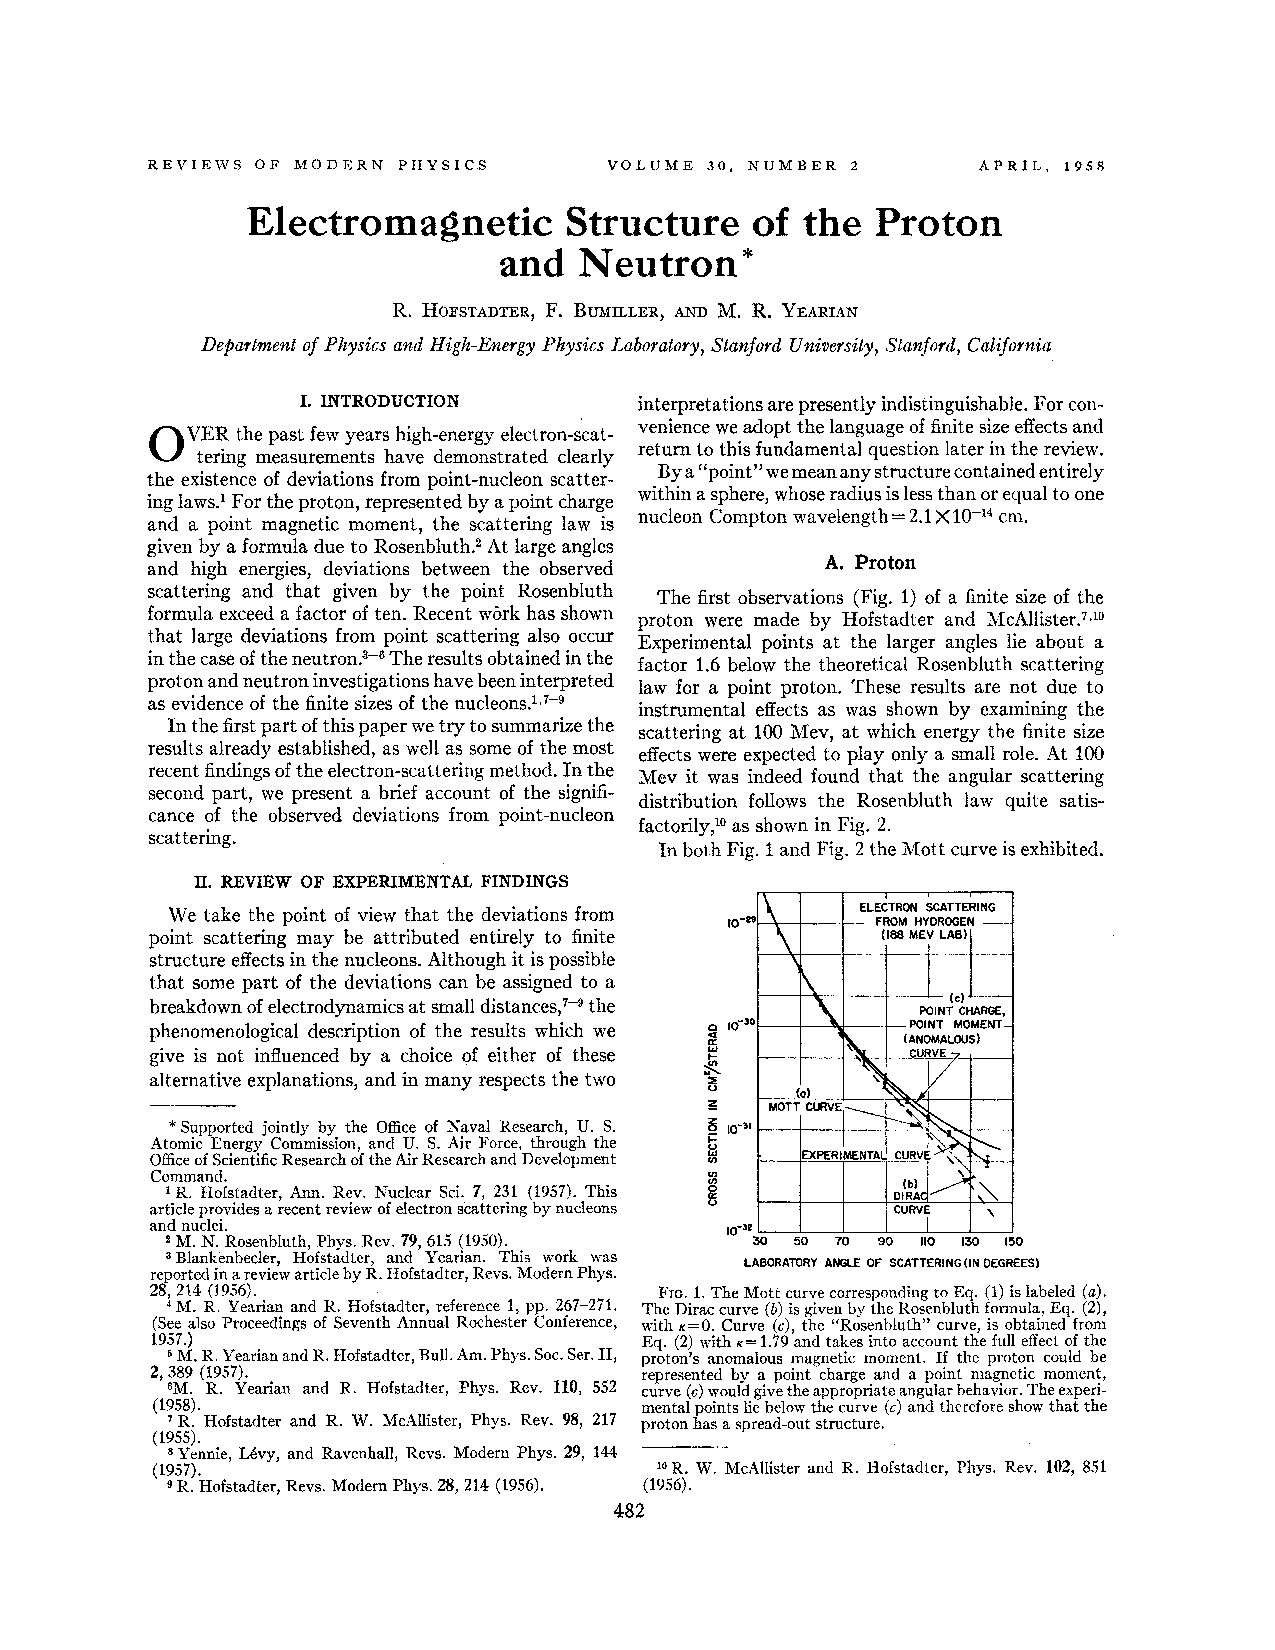
\includegraphics[width = \textwidth]{image/plots/introduction/hofstadter.pdf}	
%		\caption[Hofstadter and McAllister show that high energy electron proton scattering does not follow Rosenbluth formula.]{Hofstadter and McAllister results of scattering 188 MeV electrons from protons.  The results shown as black points disagree with predictions based on a point-like proton.  This plot motivated physicists to assert a finite size proton, and eventually study its substructure in terms of quarks and gluons.}	
%	\end{figure}

%\begin{equation}
%	\label{eqn:rosenbluth}
%	\frac{d\sigma}{d\Omega} = \frac{\alpha^2}{4 E_{1}^{2} sin^4(\theta/2)} \frac{E_3}{E_1} \left( \frac{G_{E}^2 + \tau G_{M}^2}{1 + \tau} cos^2(\theta/2) + 2 \tau G_{M}^2sin^2(\theta/2) \right)
%\end{equation}
%
%Where $\tau = \frac{Q^2}{4m_{p}^2}$.

\section{Deeply Inelastic Scattering and Structure Functions}

\begin{figure}
	\centering
	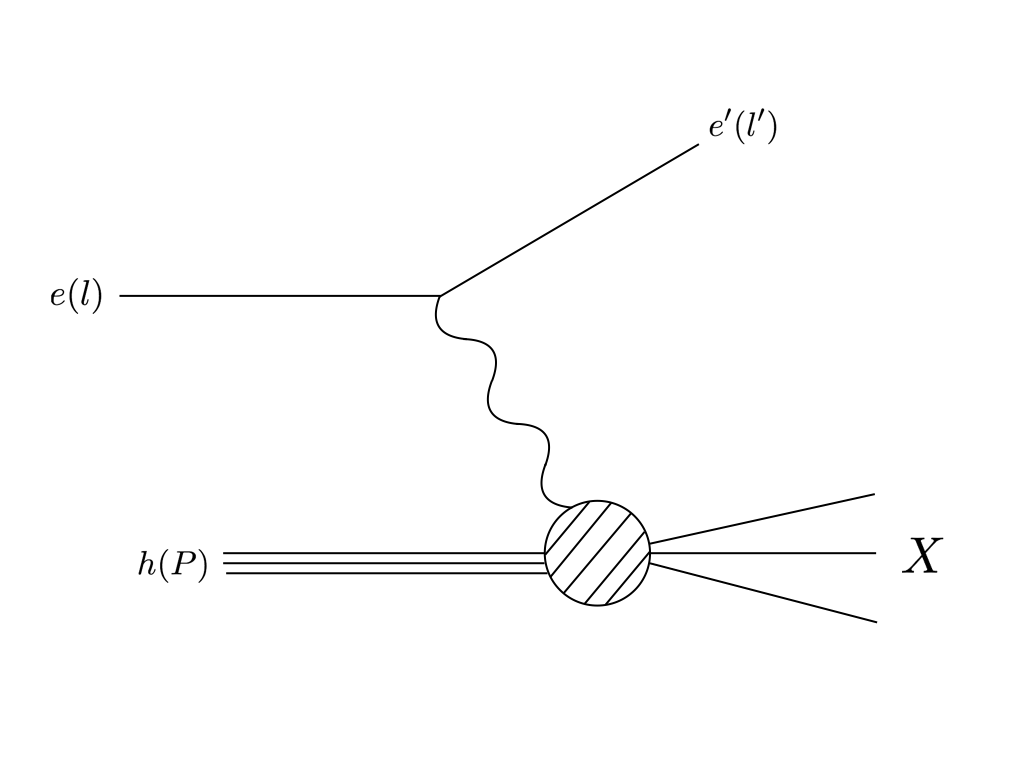
\includegraphics[width = \textwidth]{image/diagrams/dis-feynman.png}	
	\caption[A diagrammatic representation of deeply inelastic scattering.]{Deeply inelastic scattering (DIS) between a lepton and a hadron, in this thesis an electron and a proton.}
	\label{fig:dis}
\end{figure}

Learning more about quarks required scattering at higher energies.  Inelastic scattering occurs when the kinematic energy of the electron is no longer conserved, a scatterig process which dominates for $E_e \gg M_p$.  A \textit{deeply} inelastic scattering (DIS) event occurs when an electron collides with the target particle and transfers sufficient energy to interrogate it on a distance scale much smaller than its radius.  The cross section for DIS can be described using QED in terms of two structure functions $F_1$ and $F_2$.  As we will see below, these structure functions describe quark momentum in the proton.

\begin{equation}
	\label{eqn:sfs}
	\frac{d^2\sigma}{dx dQ^2} = \frac{4 \pi \alpha^2}{Q^4} \left\lbrace \left( 1 - y - \frac{m_p^2 y^2}{Q^2} \right) \frac{F_2(x,Q^2)}{x} + y^2 F_1 (x,Q^2) \right\rbrace
\end{equation}

The electron kinematics are described by the four momentum transfer $q^{\mu} = l^{\mu} - l'^{\mu}$ (shown in figure \ref{fig:dis}), the negative momentum transfer $Q^2 = - q^{\mu} q_{\mu}$ and,
\begin{align}  
  x = \frac{Q^{2}}{2P \cdot q} && y = \frac{P \cdot q}{P \cdot l} 
\end{align}

where $x$ is called the momentum fraction and $y$ is the inelasticity.  The variable $x$ (which will appear throughout this thesis) is bound between zero and one and describes the fraction of the total proton momentum carried by the quark struck in the scattering.  For the case that $Q^2 \gg m_p^2 y^2$ the cross section can be approximated as shown below.

\begin{equation}
	\label{eqn:sfs2}
	\frac{d^2\sigma}{dx dQ^2} \approx \frac{4 \pi \alpha^2}{Q^4} \left\lbrace \left( 1 - y \right) \frac{F_2(x,Q^2)}{x} + y^2 F_1 (x,Q^2) \right\rbrace
\end{equation}

First measurements of the DIS structure functions \cite{history-bjorken:1969} showed that they are approximately independent of $Q^2$ (Bjorken scaling) and that they appear to be related to each other through the Callan-Gross relation \ref{eqn:callan-gross}.

\begin{equation}	
	F_{2} (x) = 2xF_1 (x)
	\label{eqn:callan-gross}
\end{equation}

Both of these features are predicted by the parton model, a tool introduced by Richard Feynman in 1969 \cite{history-feynman:1969}.

\section{The Parton Model and Parton Distribution Functions}

\begin{figure}
	\centering
	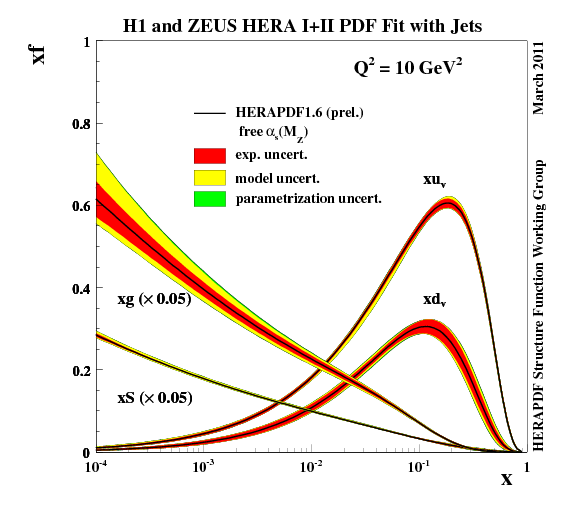
\includegraphics[width = \textwidth]{image/plots/introduction/pdf.png}	
	\caption[A recent PDF extraction from HERA data.]{PDFs extracted from HERA data, showing the dominance of gluons and sea quarks at lower momentum fraction $x$.}
	\label{fig:pdfs}
\end{figure}

Feynman noted that high energy electron-proton collisions exist on a very short timescale, and can be imagined as electrons interacting electromagnetically (or electroweakly) with single quarks in the proton.  Elastic electron-quark scattering is calculable, but since the quark in the proton is not free a parton distribution function $q_i(x)$ was introduced to model the quarks interaction with the other constituents of the proton (the index $i$ refers to the quark flavor).  Simply put, the parton distribution functions (PDFs) describe the probability of finding a quark of flavor $i$ in a proton (or other hadron) with momentum fraction $x$ (this interpretation is no longer valid once the $Q^2$ evolution is calculated using DGLAP).  By using the parton model the DIS cross section can be predicted in terms of the PDFs.    

\begin{equation}
	\label{eqn:sfs-pdf}
	\frac{d^2\sigma}{dx dQ^2} = \frac{4 \pi \alpha^2}{Q^4} \left\lbrace 1 - y + \frac{y^2}{2} \right\rbrace \sum_{i} Q_i^2 q_i^p (x)
\end{equation}

When equating \ref{eqn:sfs2} with \ref{eqn:sfs-pdf} Bjorken scaling and the Callan-Gross relation are predicted by the parton model.

\begin{equation}
	\label{eqn:bjorken-scaling}
	F_{2} (x, Q^2) = 2xF_1 (x, Q^2) = x \sum_{i} Q_i^2 q_i^p(x)
\end{equation}

These first triumphs of the parton model lead to in depth studies of the structure functions at HERA.

\section{HERA}

% Most epic figure that exists in all of 
% nucleon structure research.
\begin{figure}
	\centering
	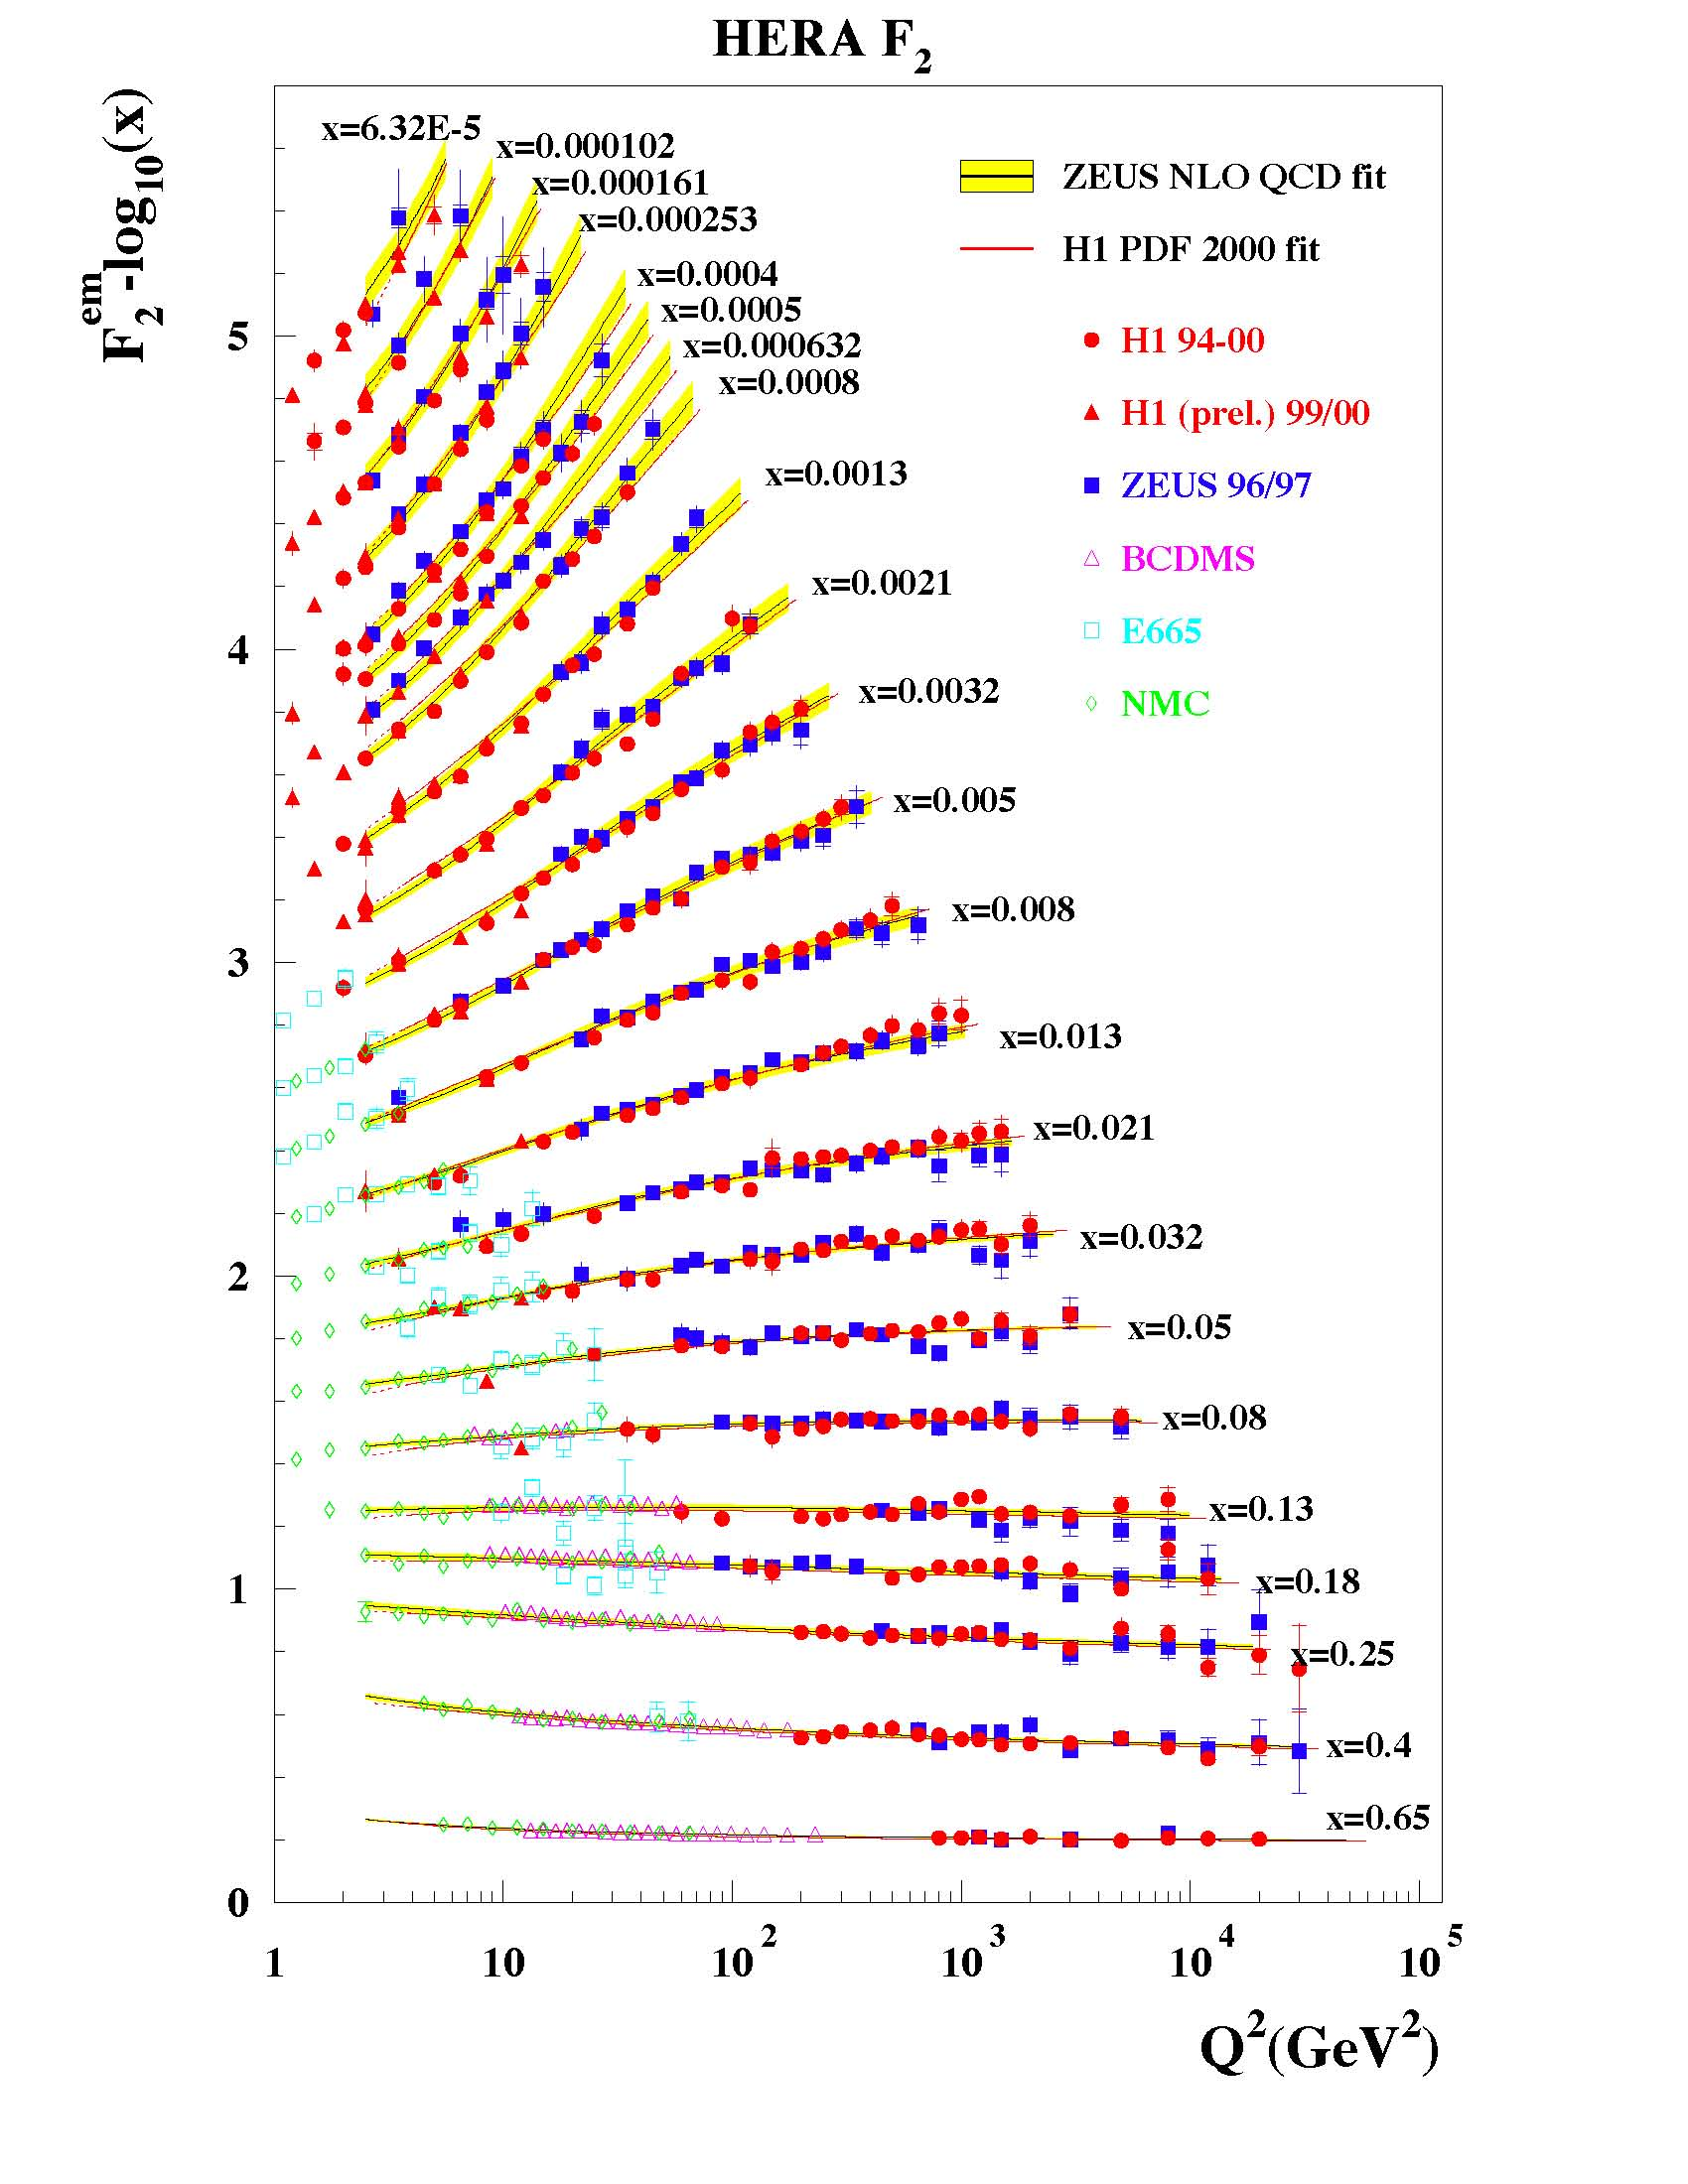
\includegraphics[width = \textwidth]{image/plots/introduction/f2.jpg}	
	\caption[$F_{2} (Q^2)$ results from HERA]{HERA experiments ZEUS and H1 mapped out the structure function $F_2$, which displayed the predicted Bjorken scaling for most values of $x$.   The mild $Q^2$ dependence of the PDFs can be calculated using the DGLAP evolution equations for the PDFs, providing an understanding for the observed dependence.}
	\label{fig:f2}
\end{figure}

HERA studied DIS extensively at large $Q^2 > 200 \; GeV^2$ by colliding 27.5 GeV electrons and 820 or 920 GeV protons.  The H1 and ZEUS experiments mapped proton structure functions in great detail.  The results \ref{fig:f2} display a weak dependence on $Q^2$; a feature calculable using the DGLAP evolution equations.  The PDFs extracted \ref{fig:pdfs} from these structure functions show that almost half of the proton momentum is carried by gluons (and quark/anti-quark pairs).  These results demonstrated that a simple picture of the proton as three valence quarks $(uud)$ is not sufficient.    

\section{Semi-Inclusive Deeply Inelastic Scattering}
DIS events where one hadron is detected in the final state are called semi-inclusive DIS (SIDIS) events.  The detection of a hadron in the final state provides information needed to go beyond a discussion of quark momentum along the hard scattering direction and into the plane transverse to it.  A diagrammatic representation of the reaction \ref{fig:sidis} shows the hadron scattering out of the lepton plane with angle $\phi$ (also noted $\phi_h$ in other places).

\begin{figure}
	\centering
	\label{fig:sidis}
	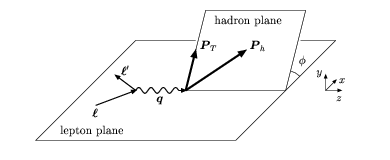
\includegraphics[width = \textwidth]{image/diagrams/phi-hadron.png}	
	\caption[Diagrammatic representation of SIDIS with hadronic $\phi_h$ angle.]{In a SIDIS event the scattered electron is detected as well as one final state hadron, allowing for the calculation of the angle $\phi_h$ which appears frequently in the SIDIS cross section.}
\end{figure}

Analogously to the manner in which the DIS cross section can be described by structure functions, the SIDIS cross section \ref{e:crossmaster} can be decomposed into a set of 18 structure functions (depending on the polarization direction of the electron and proton) \cite{tmds-mulders:1995}, \cite{tmds-bacchetta:2006}.  The structure functions $F_{ij}$ are indexed by the beam polarization $i$ and the target polarization $j$, which take on values of U, L, and T for unpolarized, longitudinal, and transverse respectively.

\begin{eqnarray}
\frac{d\sigma}{dx_B \, dy\, d\phi_s \,dz\, d\phi_h\, d p_{h\perp}^2}
&=&\frac{\alpha^2}{2x_B y Q^2}
\frac{y^2}{1-\varepsilon}  ( 1+\frac{\gamma^2}{2x_B} ) \Bigl\{  \nonumber \\
&& F_{UU ,T} +  \varepsilon F_{UU ,L}
+ \sqrt{2\,\varepsilon (1+\varepsilon)} \cos\phi_h F_{UU}^{\cos\phi_h}
+ \varepsilon \cos(2\phi_h) F_{UU}^{\cos 2\phi_h} \nonumber \\
&+& \lambda_e
\sqrt{2\,\varepsilon (1-\varepsilon)} \sin\phi_h F_{LU}^{\sin\phi_h}
+ \lambda \big[ \sqrt{2 \varepsilon (1+\varepsilon)} \sin\phi_h F_{UL}^{\sin\phi_h}
  +  \varepsilon \sin(2\phi_h) F_{UL}^{\sin 2\phi_h} \big] \nonumber \\
&+&  \lambda_e \lambda
\big[\sqrt{1-\varepsilon^2} F_{LL}
  +\sqrt{2\varepsilon (1-\varepsilon)} \cos\phi_h F_{LL}^{\cos \phi_h}\big] \nonumber \\
&+& s_\perp
\big[ \sin(\phi_h-\phi_S) \bigl(F_{UT ,T}^{\sin(\phi_h -\phi_S)}
  + \varepsilon\, F_{UT ,L}^{\sin(\phi_h -\phi_S)}\bigr) \nonumber \\
  && \phantom{s_\perp}
  + \varepsilon \sin(\phi_h+\phi_S) F_{UT}^{\sin(\phi_h +\phi_S)}
  + \varepsilon \sin(3\phi_h-\phi_S) F_{UT}^{\sin(3\phi_h -\phi_S)} \nonumber \\
  && \phantom{s_\perp}
  + \sqrt{2\,\varepsilon (1+\varepsilon)} \sin\phi_S F_{UT}^{\sin \phi_S }
  + \sqrt{2\,\varepsilon (1+\varepsilon)} \sin(2\phi_h-\phi_S) F_{UT}^{\sin(2\phi_h -\phi_S)}\big]\nonumber \\
&+& \lambda_e s_\perp
\big[\sqrt{1-\varepsilon^2} \cos(\phi_h-\phi_S) F_{LT}^{\cos(\phi_h -\phi_S)}
  +\sqrt{2\varepsilon (1-\varepsilon)} \cos\phi_S F_{LT}^{\cos \phi_S} \nonumber \\
  && \phantom{\lambda_e s_\perp}
  +\sqrt{2\,\varepsilon (1-\varepsilon)} \cos(2\phi_h-\phi_S) F_{LT}^{\cos(2\phi_h - \phi_S)} \big] \Bigr\},
\label{e:crossmaster}
\end{eqnarray}

In the SIDIS cross section the following hadronic kinematic variables are used. 

\begin{align}
  z = \frac{P \cdot P_{h}}{P \cdot q} && \gamma = \frac{2Mx}{Q}
\end{align}

Additionally, the ratio $\varepsilon$ of the longitudinal and transverse photon flux is shown below.

\begin{equation}
	\varepsilon = \frac{1 - y - \frac{1}{4}\gamma^2 y^2}{1 - y + \frac{1}{2}y^2 + \frac{1}{4}\gamma^2 y^2}
\end{equation}

By experimentally controlling the spin of the electron ($\lambda_e$) and proton different terms of the cross section can be observed in isolation.  For the remainder of this thesis our discussion will focus on unpolarized protons, reducing the number of structure functions to five.  
\begin{eqnarray}
\frac{d\sigma}{dx_B \, dy\, d\phi_s \,dz\, d\phi_h\, d p_{h\perp}^2}
&=&\frac{\alpha^2}{2x_B y Q^2}
\frac{y^2}{1-\varepsilon}  ( 1+\frac{\gamma^2}{2x_B} ) \Bigl\{  \nonumber \\
&& F_{UU ,T} +  \varepsilon F_{UU ,L}
+ \sqrt{2\,\varepsilon (1+\varepsilon)} \cos\phi_h F_{UU}^{\cos\phi_h}
+ \varepsilon \cos(2\phi_h) F_{UU}^{\cos 2\phi_h} \nonumber \\
&+& \lambda_e
\sqrt{2\,\varepsilon (1-\varepsilon)} \sin\phi_h F_{LU}^{\sin\phi_h}\Bigr\}
\end{eqnarray}

The SIDIS structure functions are actively being studied for their connection to transverse momentum dependent functions.

\section{Transverse Momentum Dependent Functions}
Two types of transverse momentum dependent functions contribute to the SIDIS structure functions.  First, encoding the quark momentum in the proton information are the transverse momentum dependent parton distribution functions (TMD PDFs), which depend on the momentum fraction $x$ as well as the quark momentum in the transverse plane $f^{a}(x, k_{T}^{2})$.  The fragmentation functions describe the probability of a quark flavor $a$ fragmenting into the observed hadron $h$ and are denoted by $D^{a}(z, p_{T}^{2})$.  At leading order (called twist-two) there are eight TMD PDFs and eight TMD FFs (see table \ref{table:twist-two-pdfs} for a list of twist two PDFs).  At twist-three an additional sixteen TMD PDFs are introducted, supressed by a factor of $M_p/Q$.

\begin{figure}
	\centering
	\begin{tabular}{|c|c|c|c|}
		\hline 
		nucleon / quark & U & L & T \\
		\hline
		U & $f_1$ & & $h_1^{\perp}$ \\
		L & & $g_{1L}$ & $h_{1L}^{\perp}$ \\
		T & $f_{1T}^{\perp}$ & $g_{1T}$ & $h_1$, $h_{1T}^{\perp}$ \\ 
		\hline
	\end{tabular}
	\caption[Twist two PDFs]{Twist two PDFs.  The leftmost column refers to the polarization of the nucleon, while the top row refers to the polarization of the quark inside of the nucleon.}
	\label{table:twist-two-pdfs}
\end{figure}

In the TMD framework, the structure functions can be expressed as convolutions of PDFs and FFs.  The following notation $\mathcal{C}[\omega f D]$ was introduced in \cite{tmds-bacchetta:2006} to simplify life.

\begin{equation}
  \mathcal{C}[\omega f D] = x \sum_{a} e^{2}_{a} \int d^{2}\pt d^{2}\kt \delta^{(2)} \left( z\kt + \pt - \vect{P}_{h\perp} \right) \omega (\kt, \pt) f^{a}(x, k_{T}^{2}) D^{a}(z, p_{T}^{2}) 
\end{equation}

The convolution operation is denoted by the $\mathcal{C}$ charactor, while the $w$ refers to a kinematic weighting function which can be one, $f$ is the PDF and $D$ is the FF.  USing this notation, the five structure functions appearing in the cross section are shown below.

\begin{equation}
F_{UU,T} = \mathcal{C}[f_1 D_1] = x \sum_{a} e^{2}_{a} \int d^{2} \pt d^{2} \kt \delta^{(2)} \left( z\kt + \pt - \vect{P}_{h\perp} \right) f_{1}^{a}(x, k_{T}^{2}) D_{1}^{a}(z, p_{T}^{2})
\end{equation}

\begin{equation}
F_{UU,L} = 0
\end{equation}

\begin{equation}
F_{UU}^{\cos \phi_h} = \frac{2M}{Q} \mathcal{C} \Bigl[ - \frac{\hhat \cdot \kt}{M_h} \Bigl( x h H_{1}^{\perp} + \frac{M_h}{M} f_1 \frac{\tilde{D}^{\perp}}{z} \Bigr) - \frac{\hhat \cdot \pt}{M} \Bigl( x f^{\perp} D_1 + \frac{M_h}{M} h_1^{\perp} \frac{\tilde{H}}{z} \Bigr)\Bigr]
\end{equation}

\begin{equation}
F_{UU}^{\cos 2\phi_h} = \mathcal{C} \Bigl[ - \frac{2 (\vect{\hat{h}} \cdot \kt) (\vect{\hat{h}} \cdot \pt) - \kt \cdot \pt}{M M_h} h_{1}^{\perp} H_{1}^{\perp} \Bigr]
\end{equation}

\begin{equation}
  F_{LU}^{\sin\phi} = \frac{2M}{Q} \mathcal{C} \Bigl[ -\frac{\hhat \cdot \kt}{M_h} \Bigl( xeH_1^\perp + \frac{M_h}{M} f_1 \frac{\tilde{G}^\perp}{z} \Bigr) + \frac{\hhat \cdot \pt}{M} \Bigl( xg^\perp D_1 + \frac{M_h}{M} h_{1}^{\perp} \frac{\tilde{E}}{z} \Bigr) \Bigr]
\end{equation}

%  Possible extensions: are they MVP?
%     - Brief discussion of assumptions, factorization
%     - Discussion of the techniques for measuring SFs and extracting PDFs and FFs (this paints
%       a better motivation for my efforts in measuring two different things to a larger more 
%       difficult effort.

\section{This Thesis}
This work presents two novel SIDIS measurements.  A measurement of beam spin asymmetries (BSA) for positively charged k-mesons (kaons or $K^+$) is presented in chapter 8.  The BSA is defined as, 

\begin{equation}
  BSA = \frac{d\sigma^+ - d\sigma^-}{d\sigma^+ + d\sigma^-} = \frac{\phimod{LU}{\sin\phi}}{1 + \phimod{UU}{\cos\phi} + \phimod{UU}{\cos(2\phi)}}
\end{equation}

where the coefficient $A_{LU}^{\sin\phi}$ is shown below.

\begin{equation}
  A_{LU}^{\sin\phi} = \sqrt{2\,\varepsilon (1-\varepsilon)} \frac{F_{LU}^{\sin\phi}}{F_{UU,T} + \varepsilon F_{UU,L}}
\end{equation}

The unpolarized cross section for charged pions ($\pi^{\pm}$) is also presented in chapter 7.  This analysis extends the work of Nathan Harrison in his thesis work \cite{theses-harrison:2015}.

%	% 10. Wes Gohn 
%	Recently CLAS reported the non-zero BSA measurement of charged and neutral pion beam spin asymmetries, which implies that in the kinematics measured by CLAS, the twist three TMD terms cannot be neglected [reference to Wes Gohn thesis].  As a natural extension of this knowledge, I analyze the same observable for the heavier kaon channel to see if the same conclusion is realized.

% Structural overview of thesis 
I have reviewed the experimental hardware that enables this thesis work in chapter 2 and summarized analytical techniques used during chapter 3.  I describe basic analysis procedures that are common to both measurements in chapter 4 before discussing particle identification in chapter 5.  I present results for the inclusive scattering cross section in chapter 6, followed by the SIDIS cross section in chapter 7.  I then present my findings for the positively charged kaon BSA measurement in chapter 8 before offering a brief summary and outlook in chapter 9. 

